\documentclass{article}
\usepackage[UTF8]{ctex}
\usepackage{newtxtext}
\usepackage{geometry}
\usepackage[dvipsnames,svgnames]{xcolor}
\usepackage[strict]{changepage} % 提供一个 adjustwidth 环境
\usepackage{framed} % 实现方框效果
\usepackage{setspace}
\usepackage{tikz}
\usepackage{tcolorbox}
\usepackage{amsmath}
\usepackage{graphicx}
\usepackage{wrapfig}
\usepackage{float}
\usepackage{amssymb}
\geometry{a4paper,centering,scale=0.8,left=2.0cm,right=2.0cm,top=2.0cm,bottom=2.0cm}

\definecolor{blueshade}{rgb}{0.95,0.95,1} % 文%本框颜色
\definecolor{greenshade}{rgb}{0.90,0.99,0.91} % 绿色文本框,竖线颜色设为 Green
\definecolor{redshade}{rgb}{1.00,0.90,0.90}% 红色文本框,竖线颜色设为 LightCoral
\definecolor{brownshade}{rgb}{0.99,0.97,0.93} % 莫兰迪棕色,竖线颜色设为 BurlyWood
\definecolor{yellowshade}{rgb}{1,0.945,0.7255}%米黄色
\definecolor{DarkYellow}{rgb}{0.7843,0.61176,0.0549}

\newenvironment{formal}[2][greenshade]{%
\def\FrameCommand{%
\hspace{1pt}%
{\color{#2}\vrule width 2pt}%
{\color{#1}\vrule width 4pt}%
\colorbox{#1}%
}%
\MakeFramed{\advance\hsize-\width\FrameRestore}%
\noindent\hspace{-4.55pt}% disable indenting first paragraph
\begin{adjustwidth}{}{7pt}%
\vspace{2pt}\vspace{2pt}%
}
{
\vspace{2pt}\end{adjustwidth}\endMakeFramed%
}



\title{\Huge 证券投资学-第二次作业    \\\large made by  \LaTeX}
\author{刘宇晨\hspace*{25pt}20002515\\计金(双)200}


%\begin{tcolorbox}
%    [colback=Emerald!10,colframe=cyan!40!black,title=\textbf{公式}]
%\end{tcolorbox}

\begin{document} 
\begin{figure}[H]
    \begin{center}
        
\includegraphics[width=0.3\textwidth]{logo.jpeg}
        \maketitle
    \end{center}
\end{figure}
\thispagestyle{empty}
\clearpage
\pagenumbering{arabic}
\section*{\center 第八章作业}
\subsection*{习题6}
\begin{spacing}{0.9}
    构建单因素模型,需要的变量:
    \begin{itemize}
        \item $n(\mathcal{A} ,\mathcal{B} )$个超额收益估计值,$\alpha_\mathcal{A}=13\%-8\% ,\alpha_\mathcal{B}=18\%-8\%$
        \item $n(\mathcal{A} ,\mathcal{B} )$个敏感系数估计值,$\beta_\mathcal{A}=0.8,\beta_\mathcal{B}=1.2 $
        \item $n(\mathcal{A} ,\mathcal{B} )$个公司特有方差的估计值,$\sigma^2(e_\mathcal{A} )=30\%,\sigma^2(e_\mathcal{B} )=40\%$
        \item 1个市场溢价估计值,$E(R_M)=\text{UNKNOWN}$
        \item 1个宏观经济因素方差的估计值,$\sigma_M^2=22\%$
    \end{itemize}
\end{spacing}


a.股票$\mathcal{A} $和$\mathcal{B} $的标准差(总风险)
\nonumber
\begin{align}
    \text{总风险}&=\text{系统性风险}+\text{公司特定风险}\\
    \sigma_i^2&=\beta_i^2\sigma_M^2+\sigma^2(e_i)\\
    \sigma_\mathcal{A}=\sqrt{ \sigma_\mathcal{A} ^2}&=\sqrt{\beta_\mathcal{A} ^2\sigma_M^2+\sigma^2(e_\mathcal{A} )}=\sqrt{0.8^2\times 0.22^2+0.3^2}=34.78\%\\
    \sigma_\mathcal{B}=\sqrt{\sigma_\mathcal{B} ^2}&=\sqrt{\beta_\mathcal{B} ^2\sigma_M^2+\sigma^2(e_\mathcal{B} )}=\sqrt{1.2^2\times 0.22^2+0.4^2}=347.93\%
\end{align}

b.计算期望收益率、标准差、$\beta$和非系统性标准差(公司特定标准差)
\begin{tcolorbox}
    [colback=Emerald!10,colframe=cyan!40!black,title=\textbf{$\sigma_P$是标准差,$\sigma(e_P)$是非系统性标准差}]
    \nonumber
    \begin{align}
        E(r_P)&=w_\mathcal{A} \times E(r_\mathcal{A} )+w_\mathcal{B} \times E(r_\mathcal{B})+w_f\times r_f\\
        &=0.3\times 0.13+0.45\times 0.18+0.25\times 0.08=14\%\\
        \beta_P&=w_\mathcal{A} \times \beta_\mathcal{A}+w_\mathcal{B} \times \beta_\mathcal{B}\\
        &=0.3\times 0.8+0.45\times 1.2=0.78\\
        \sigma^2(e_P)&=w_\mathcal{A} \times \sigma^2(e_\mathcal{A} )+w_\mathcal{B} \times \sigma^2(e_\mathcal{B} )\\
                &=0.30^2\times 0.30^2+0.45^2\times 0.40^2=4.05\%\\
        \sigma(e_P)=\sqrt{\sigma^2(e_P)}&=\sqrt{4.05\%}=20.12\%\\
        \sigma_P^2&=\beta_P^2\sigma_M^2+\sigma^2(e_P)\\
        &=(0.78^2+0.22^2)+4.05\%=6.99\%\\
        \sigma_P=\sqrt{\sigma_P^2}&=\sqrt{6.99\%}=26.45\%
    \end{align}
\end{tcolorbox}
\clearpage

\section*{习题8}
\begin{spacing}{0.9}
    构建单因素模型,需要的变量:
    \begin{itemize}
        \item $n(\mathcal{A} ,\mathcal{B} )$个超额收益估计值,$\alpha_\mathcal{A}=1\% ,\alpha_\mathcal{B}=-2\%$
        \item $n(\mathcal{A} ,\mathcal{B} )$个敏感系数估计值,$\beta_\mathcal{A}=1.2,\beta_\mathcal{B}=0.8$
        \item $n(\mathcal{A} ,\mathcal{B} )$个公司特有方差的估计值,$\sigma^2(e_\mathcal{A} )=10.3\%,\sigma^2(e_\mathcal{B} )=9.1\%$
        \item 1个市场溢价估计值,$E(R_M)=\text{UNKNOWN}$
        \item 1个宏观经济因素方差的估计值,$\sigma_M^2=\text{UNKNOWN}$
    \end{itemize}
\end{spacing}
a.哪个公司特定风险更高?

公司特定风险为$\sigma(e_i)$,在题目中具体表现为残差标准差,且$\sigma(e_\mathcal{A} )>\sigma(e_\mathcal{B} )$
所以$\mathcal{A} $的公司特定风险更高\\

b.哪个市场风险更高?

市场风险为系统性风险$=\beta_i^2\sigma_M^2$,$\mathcal{A} $与$\mathcal{B} $共用一个宏观经济因素$\sigma_M$(虽然题目没给),
根据条件,有$\beta_\mathcal{A} >\beta_\mathcal{B} $。所以$\beta_\mathcal{A} ^2\sigma_M^2>\beta_\mathcal{B} ^2\sigma_M^2$
。综上,$\mathcal{A} $市场风险更高\\

c.拟合优度$R^2$能解释收益整体方差中可由市场收益率解释的部分。根据条件,$R_\mathcal{A} ^2>R_\mathcal{B} ^2$。
所以$\mathcal{A} $的拟合效果更好,说明公司特定风险对整体的干扰较小,即系统性风险(市场变动)能更好地解释收益波动\\

d.假设无风险收益率为6\%,回归使用的是总收益而非超额收益,求$\mathcal{A} $的回归截距:
回归的方程是:
\[R_i=\alpha_i+\beta_iR_M\]
斜率为$\beta_i$,自变量是$R_M$,剩下的$\alpha_i$是截距,在进行变化后,除了$R_M$项都为截距项。所以:
\begin{align}
    E(R_i)&=\alpha_i+\beta_iE(R_M)\\
    r_\mathcal{A}-r_f&=\alpha_i+\beta_i(r_M-r_f)\\
    r_\mathcal{A}& =\alpha_i+r_f(1-\beta_i)+r_M\beta_i\\
  \therefore \text{截距}&=\alpha_i+r_f(1-\beta_i)\\
  &=1\%+6\%(1-1.2)=-0.2\%
\end{align}
\clearpage

\section*{习题9、10、11、12}
\begin{spacing}{0.9}
    构建单因素模型,需要的变量:
    \begin{itemize}
        \item $n(\mathcal{A} ,\mathcal{B} )$个超额收益估计值,$\alpha_\mathcal{A}=3\% ,\alpha_\mathcal{B}=-2\%$
        \item $n(\mathcal{A} ,\mathcal{B} )$个敏感系数估计值,$\beta_\mathcal{A}=0.7,\beta_\mathcal{B}=1.2$
        \item $n(\mathcal{A} ,\mathcal{B} )$个公司特有方差的估计值(之后可以通过$R^2$计算得出),$\sigma^2(e_\mathcal{A} )=\text{UNKNOWN},\sigma^2(e_\mathcal{B} )=\text{UNKNOWN}$
        \item 1个市场溢价估计值,$E(R_M)=\text{UNKNOWN}$
        \item 1个宏观经济因素方差的估计值,$\sigma_M^2=\text{UNKNOWN}$
    \end{itemize}
\end{spacing}
9.求每只股票的标准差

题目中已知拟合优度$R^2$,书中说$R^2$等于被解释的$SS$除以总的$SS$。其中,回归平方和(SS)表示因变量方差中
能够被自变量解释的那一部分,该值等于$\beta_i^2\sigma_M^2$。而总的SS等于股票的总体方差$\sigma_i^2$。所以,有:
\begin{align}
    R^2&=\frac{\beta_i^2\sigma_M^2}{\sigma_i^2}=\frac{\text{解释方差}}{\text{总体方差}}\\
    \sigma_\mathcal{A} ^2&=\beta_i^2\sigma_M^2/R_\mathcal{A} ^2=0.7^2\times 0.2^2/0.2=9.8\%\\
    \sigma_\mathcal{A}&=\sqrt{\sigma_\mathcal{A}^2}=\sqrt{9.8\%}=31.3\%\\
    \sigma_\mathcal{B} ^2&=\beta_i^2\sigma_M^2/R_\mathcal{B} ^2=1.2^2\times 0.2^2/0.12=48\%\\
    \sigma_\mathcal{B}&=\sqrt{\sigma_\mathcal{B}^2}=\sqrt{9.8\%}=69.28\%
\end{align}

10.将总方差分解为系统性和公司特定的两部分
\begin{align}
    \text{总风险}&=\text{系统性风险}+\text{公司特定风险}\\
    \sigma_i^2&=\beta_i^2\sigma_M^2+\sigma^2(e_i)\\
    \mathcal{A} \text{系统风险}&=\beta_\mathcal{A} ^2\sigma_M^2=0.7^2\times 0.2^2=1.96\%\\
    \mathcal{A} \text{公司特有风险}&=\sigma^2(e_\mathcal{A} )=\sigma_\mathcal{A} ^2-(\beta_\mathcal{A} ^2\sigma_M^2)=9.8\%-1.96\%=7.84\%\\
    \text{同理}&\text{,}\\
    \mathcal{B} \text{系统风险}&=\beta_\mathcal{B} ^2\sigma_M^2=1.2^2\times 0.2^2=5.76\%\\
    \mathcal{B} \text{公司特有风险}&=\sigma^2(e_\mathcal{B} )=\sigma_\mathcal{B} ^2-(\beta_\mathcal{B} ^2\sigma_M^2)=48\%-5.76\%=42.24\%
\end{align}

11.求两只股票之间的协方差和相关系数
\begin{align}
    \text{协方差}&=\beta\text{的乘积}\times\text{市场指数风险}\\
    \text{Cov}(r_\mathcal{A} ,r_\mathcal{B} )&=\beta_\mathcal{A} \beta_\mathcal{B} \sigma_M^2\\
    &=0.7\times 0.12\times (20\%)^2=3.36\%\\
    \text{相关系数}&=\text{与市场之间的相关系数之积}\\
    \text{Corr}(r_\mathcal{A} ,r_\mathcal{B})&=\frac{\beta_\mathcal{A} \beta_\mathcal{B} \sigma_M^2}{\sigma_\mathcal{A} \sigma_\mathcal{B}}=\frac{0.7\times 1.2\times(20\%)^2}{\sqrt{9.8\%\times 48\%}}=0.155
\end{align}

12.每只股票与市场指数的协方差是多少
\begin{align}
    \text{Cov}(r_\mathcal{A} ,r_M )&=\beta_\mathcal{A}  \beta_M \sigma_M^2=0.7\times 1\times 20\%^2=2.8\%\\
    \text{Cov}(r_\mathcal{B} ,r_M )&=\beta_\mathcal{B}  \beta_M \sigma_M^2=1.2\times 1\times 20\%^2=4.8\%
\end{align}
\clearpage

\subsection*{习题16}
根据教材最后风险组合构造程序,分别将股票$\mathcal{A} .\mathcal{B} $作为积极组合进行构造:
\subsubsection*{方法一}
\begin{enumerate}
    \item 计算积极组合中每个证券的原始头寸:由于分别进行构造,所以不必构造原始头寸
    \item 调整这些原始权重,使组合权重和为1,略过
    \item 计算积极组合的$\alpha$值:
    \begin{align}
        E(R_i)&=\alpha_i+\beta_iE(R_M)\\
        \alpha_\mathcal{A} &=E(R_i)-\beta_iE(R_M)=0.2\%\\
        \alpha_\mathcal{B} &=E(R_i)-\beta_iE(R_M)=-1\%
    \end{align}
    \item 计算积极组合的残差:$\sigma^2(e_\mathcal{A} )=10\%^2,\sigma^2(e_\mathcal{B} )=11\%^2$
    \begin{align}
        \text{公司特定风险}&=\text{总风险}-\text{系统性风险}\\
        \sigma^2(e_i)&=\sigma_i^2-\beta_i^2\sigma_M^2\\
        \sigma^2(e_\mathcal{A} )&=10\%^2-0.8^2\times 5\%^2=0.84\\
        \sigma^2(e_\mathcal{B} )&=11\%^2-0.8^2\times 5\%^2=0.6475
    \end{align}
    \item 计算积极组合原始头寸:
    \begin{align}
        w_i^0&=\frac{\alpha_i \sigma_M^2}{E\left(R_M\right) \sigma^2(e_i)}\\
        w_\mathcal{A} ^0&=\frac{0.2\% \times 5\%^2}{(12\%-6\%)\times 0.84\%}=0.0099\\
        w_\mathcal{B} ^0&=\frac{-1\% \times 5\%^2}{(12\%-6\%)\times 0.6475\%}=-0.06435\\
    \end{align}
    \item 计算积极组合$\beta$值:$\beta_\mathcal{A} =0.8,\beta_\mathcal{B} =1.5$
    \item 调整积极组合的原始头寸:
    \begin{align}
        w_i ^*&=\frac{w_i ^0}{1+(1-\beta_i ) w_i ^0}\\
        w_\mathcal{A} ^*&=\frac{0.0099}{1+(1-0.8)0.0099}=0.988\%\\
        w_\mathcal{B} ^*&=\frac{-0.06435}{1+(1-1.5)(-0.06435)}=-6.2344\%
    \end{align}
    \item 此时最优风险组合的权重:$w_M^*=1-w_i^*$\\
    选择一:由于$w_\mathcal{A} ^*>w_\mathcal{B} ^*$,故可以选择做多$\mathcal{A} $
    选择二:由于$|w_\mathcal{B} ^*|>|w_\mathcal{A} ^*|$,故可以选择做空$\mathcal{B} $
\end{enumerate}
\clearpage
\subsubsection*{方法二}
积极组合(当持有最优权重时)对整个风险投资组合的夏普比率的贡献取决于它的$\alpha$值和残差标准差的比率。
所以此题可以分别计算$\mathcal{A} ,\mathcal{B} $的信息比率来进行判断。
\begin{align}
    S_P^2&=S_M^2+{[\frac{\alpha_A}{\sigma(e_A)}]}^2\\
    E(R_i)&=\alpha_i+\beta_iE(R_M)\\
    \alpha_\mathcal{A} &=E(R_i)-\beta_iE(R_M)=0.2\%\\
    \alpha_\mathcal{B} &=E(R_i)-\beta_iE(R_M)=-1\%\\
    \text{公司特定风险}&=\text{总风险}-\text{系统性风险}\\
    \sigma^2(e_i)&=\sigma_i^2-\beta_i^2\sigma_M^2\\
    \sigma^2(e_\mathcal{A} )&=10\%^2-0.8^2\times 5\%^2=0.84\\
    \sigma^2(e_\mathcal{B} )&=11\%^2-0.8^2\times 5\%^2=0.6475\\
    \mathcal{A} \text{的}S_P^2&={\frac{12\%-6\%}{6\%}}^2+{[\frac{0.2\%}{\sqrt{0.84}}]}^2=0.360476\%\\
    \mathcal{B} \text{的}S_P^2&={\frac{12\%-6\%}{6\%}}^2+{[\frac{-1\%}{\sqrt{0.6475}}]}^2=0.37544\%
\end{align}
由于$\mathcal{B} $的信息比率大于$\mathcal{A} $的信息比率,且$\mathcal{B} $的$\alpha<0$,所以选择做空$\mathcal{B} $
\clearpage
\section*{\center 第九章作业}
\subsection*{习题9}
a.假设激进型股票为$\mathcal{A} $,防守型股票为$\mathcal{B} $,根据题目和期望收益-贝塔关系,有
\begin{align}
    E(r_P)&=r_f+\beta_P[E(r_M)-r_f]\\
    \text{对于股票}\mathcal{A} &
    \begin{cases}
        E(r_{P1})=r_f+\beta_\mathcal{A} [E(r_{M1})-r_f]\Rightarrow -2\%=r_f+\beta_\mathcal{A} (5\%-r_f)\\
        E(r_{P2})=r_f+\beta_\mathcal{A} [E(r_{M2})-r_f]\Rightarrow 38\%=r_f+\beta_\mathcal{A} (25\%-r_f)
    \end{cases}\\
    \text{解得:}&
    \begin{cases}
        \beta_\mathcal{A} =2\\
        r_f=12\%
    \end{cases}\\
    \hline
    \text{对于股票}\mathcal{B} &
    \begin{cases}
        E(r_{P1})=r_f+\beta_\mathcal{B} [E(r_{M1})-r_f]\Rightarrow 6\%=r_f+\beta_\mathcal{B} (5\%-r_f)\\
        E(r_{P2})=r_f+\beta_\mathcal{B} [E(r_{M2})-r_f]\Rightarrow 12\%=r_f+\beta_\mathcal{B} (25\%-r_f)
    \end{cases}\\
    \text{解得:}&
    \begin{cases}
        \beta_\mathcal{B} =0.3\\
        r_f=6.43\%
    \end{cases}\\
\end{align}

b.如果$P(1 )=P(2)=0.5$,则$\mathcal{A} $和$\mathcal{B} $的期望收益率:
\begin{align}
    E(r_\mathcal{A} )&=0.5\times -2\%+0.5\times 38\%=18\%\\
    E(r_\mathcal{B} )&=0.5\times 6\%+0.5\times 12\%=9\%
\end{align}
\clearpage
c.国债利率(无风险收益率)$r_f$为6\%,收益几率和b所描述的一样,求证券市场线:

描绘证券市场线:需要知道两个点,分别是$\beta_M=0$和$\beta_M=1$时,即无风险国债和市场平均收益的情况。
而且,在均衡市场中所有证券应该都在这条证券市场线上。由此经过简单的数学计算可以得知,证券市场线的
截距是无风险利率,斜率是市场平均超额收益率。对于这道题,有:
\begin{align}
    E(r_M)&=0.5\times 25\%+0.5\times 5\%=15\%\\
    \beta_f&=0,r_f=6\%\\
    \beta_M&=1,E(r_M)=15\%\\
    \text{解得SML方程:}E(r)&=6\%+\beta\times 9\%\\
    \text{对于}\mathcal{A} \text{点},\beta_\mathcal{A} &=2,E(r_\mathcal{A} )=18\%\\
    \text{对于}\mathcal{B} \text{点},\beta_\mathcal{B} &=0.3,E(r_\mathcal{A} )=9\%
\end{align}
\begin{figure}[H]
    \begin{center}
        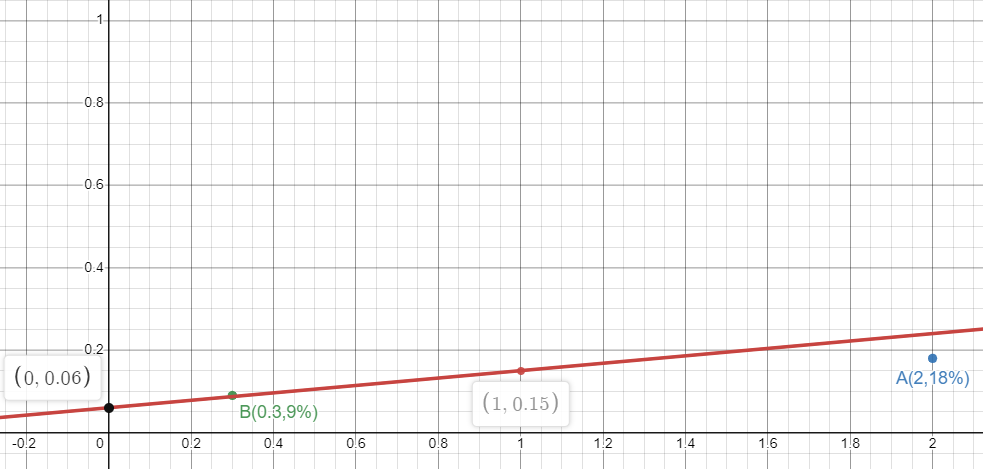
\includegraphics[width=1\textwidth]{1.png}
        \maketitle{证券市场线(Desmos)}
    \end{center}
\end{figure}

d.标出$\mathcal{A} $,$\mathcal{B} $在图中的位置(见上图),并分别求出对应的$\alpha$:

股票的实际期望收益与正常期望收益之间的差,称为股票的阿尔法($\alpha_i$)。

令$\beta$为2,在证券市场线上,收益应为$E^{\prime}(r_\mathcal{A} )=6\%+2\times 9\%=24\%$,题目中
的信息$\mathcal{A} $的期望收益率$E(r_\mathcal{A} )=18\%$,解得:
\[\alpha_\mathcal{A} =18\%-24\%=-6\%\]

同理可得:
\[\alpha_\mathcal{B} =9\%-8.7\%=0.3\%\]

e.求激进型企业的临界利率:

令激进型企业的$\beta$值等于防守型企业,$\beta=0.3$,带入证券市场线求得临界利率为8.7\%


\clearpage

\subsection*{习题20}
a.判断哪个投资者更善于选择个股

由于题目只给了两个投资者的平均收益率和$\beta$值,并没有提供无风险收益率和市场平均收益率。
故无法通过构造证券市场线的方法来计算$\alpha$值来判断谁的投资效果好。

换一种思路,可以通过判断相同风险厌恶系数下各自效用的多少来判断投资效果,但是题目只提供了$\beta$值,
并不知道两种投资的标准差,所以也无法通过计算各自的效用来判断投资效果。\\

b.已知$r_f=6\%,r_M=14\%$,判断哪个投资者选股更出色

假设两个投资者的投资组合分别是$\mathcal{A} ,\mathcal{B} $,构造证券市场线:
\begin{align}
    \text{SML方程:}E(r)&=6\%+\beta\times 14\%\\
    \text{对于}\mathcal{A} \text{点},\beta_\mathcal{A} &=1.5,E(r_\mathcal{A} )=19\%\\
    \text{对于}\mathcal{B} \text{点},\beta_\mathcal{B} &=1,E(r_\mathcal{A} )=16\%\\
    \alpha_\mathcal{A} &=(6\%+1.5\times14\%)-19\%=1\%\\
    \alpha_\mathcal{B} &=(6\%+1\times14\%)-16\%=2\%
\end{align}

有$\alpha_\mathcal{B}>\alpha_\mathcal{A}$,所以投资组合$\mathcal{B}$的异常收益更高,
书中说有人认为证券分析就是找出$\alpha$非零的证券。资产组合管理者将增加$\alpha$大于零的证券的比例,
减小$\alpha$小于零的证券的比例。所以投资组合$\mathcal{B} $要优于$\mathcal{A}$。故后者选股更出色。\\

c.已知$r_f=3\%,r_M=15\%$,判断哪个投资者选股更出色

与b.一样,假设两个投资者的投资组合分别是$\mathcal{A} ,\mathcal{B} $,构造证券市场线:
\begin{align}
    \text{SML方程:}E(r)&=3\%+\beta\times 15\%\\
    \text{对于}\mathcal{A} \text{点},\beta_\mathcal{A} &=1.5,E(r_\mathcal{A} )=19\%\\
    \text{对于}\mathcal{B} \text{点},\beta_\mathcal{B} &=1,E(r_\mathcal{A} )=16\%\\
    \alpha_\mathcal{A} &=(3\%+1.5\times15\%)-19\%=-2\%\\
    \alpha_\mathcal{B} &=(3\%+1\times15\%)-16\%=1\%
\end{align}

有$\alpha_\mathcal{B}>\alpha_\mathcal{A}$,依然是后者选股更出色。

\clearpage
\subsection*{习题21}
a.市场组合的期望收益率

在证券市场线中,因为市场的$\beta=1$,这一点就是市场投资组合的期望收益率,故
\[r_M=12\%\]

b.求$\beta=0$的股票的期望收益率

$\beta=0$的股票在证券市场线中为截距,即无风险收益,故
\[r_{\beta=0}=r_f=5\%\]

c.构造证券市场线,并求出$\beta=0.5$时证券市场线上该股票的期望收益:
\begin{align}
    \text{SML方程:}E(r)&=5\%+\beta\times 12\%\\
    \text{对于该股票},\beta_i &=1.5,E^{\prime}(r_i )=5\%+0.5\times 12\%=11\%
\end{align}

计算该股票预期的年收益率:
\begin{align}
    E(r_i)&=(\frac{41+3}{40}-1 )\times 100\% = 10\%\\
    E(r_i)&>E^{\prime}(r_i )
\end{align}

所以股票被低估了。





\end{document}